\documentclass[
	11pt, 
	a4paper, 
	twoside,
	parskip=half*, % Line spacing for paragraphs
	openany,  % openany -> on which page should new chapters start
	listof=totoc, % Include listings in the table of contents
	bibliography=totoc, % adding a bibliography to the table of contents
	index=totoc, % add index directory to the table of contents
  toc=chapterentrywithdots, % Set dots in the table of contents also for chapters
  numbers=noenddot, % removes the last dot after X.X.X.
  %chapterprefix=true % changes the display of the chapter, adds "Chapter" to the chapter number
]{scrbook}

\usepackage[utf8]{inputenc}
\usepackage[ngerman]{babel}
\usepackage{url}
\usepackage[autostyle=true,german=quotes]{csquotes}
\usepackage[T1]{fontenc}
\usepackage{pdfpages}
\usepackage{textcomp}
\usepackage{amsmath} % math environment
\usepackage[toc,acronym]{glossaries}
\usepackage{multicol}
\usepackage{listings}
%\usepackage[toc,acronym]{glossaries}  % Enable glossary and acronym list with table of contents integration
% Define Markdown language syntax
\lstdefinelanguage{markdown}{
    basicstyle=\ttfamily,
    sensitive=true,
    keywords={},
    otherkeywords={},
    morecomment=[l]{//},
    morecomment=[n]{/*}{*/},
    morestring=[b]',
    morestring=[b]",
}

% ---------------------------
% |    Meta-Data for PDF    |
% ---------------------------
\usepackage[
  pdftex,
  pdfauthor={Daniel Menzel},
  pdftitle={Thesis Template},
  pdfsubject={Bachelorthesis},
  pdfkeywords={Thesis;Template;LaTeX},
  pdfproducer={LaTeX},
  pdfcreator={pdfLaTeX},
  pdfduplex={DuplexFlipLongEdge}, %Alt.: Simplex or DuplexFlipShortEdge 
  pdflang={de}, % en
  bookmarksopen,
  bookmarksnumbered,
]{hyperref}

% ------------------
% |    Settings    |
% ------------------
\usepackage[
    backend=biber,
    style=ieee,        % Sets bibliography and citation style to IEEE
    maxnames=3,        % Maximum number of authors before "et al." is used, typically more than 1 for IEEE
    isbn=false,        % Typically ISBN is not included in IEEE papers
    doi=true,          % Display DOI as it's common in IEEE citations
    url=true,          % Display URLs as they can be important in IEEE citations
    eprint=false       % Eprints are usually not included in IEEE
]{biblatex}

% Set distance between bibliographical references
\setlength{\bibitemsep}{.5em}

% Set indentation for each bibliographic entry
\setlength{\bibhang}{2em}

% Format URLs in the bibliography to be within angle brackets
\DeclareFieldFormat{url}{<\url{#1}>}

% Set penalties for breaking URLs to prevent overfull boxes
\setcounter{biburllcpenalty}{7000}
\setcounter{biburlucpenalty}{8000}

% Source of the bibliography file
\addbibresource{sources/literature.bib} % .bib extension is required here
% graphics
\usepackage{graphicx}
\graphicspath{ {images/} }
\DeclareGraphicsExtensions{.pdf,.png,.jpg,.jpeg,.gif}

% captions
\usepackage{caption}
\usepackage{subcaption}
% Table layout
\setlength{\tabcolsep}{0.5em} % for the horizontal padding
{\renewcommand{\arraystretch}{1.2} % for the vertical padding

% Table captions
\usepackage{caption} 
\captionsetup[table]{belowskip=12pt,aboveskip=4pt}
\usepackage{diagbox}

% Rotate tables
\usepackage{rotating}
\usepackage{varwidth}

% Footnotes with tables
\usepackage{footnote}
\makesavenoteenv{figure}

% Line breaks in table cells
\newcommand{\specialcell}[2][c]{%
  \begin{tabular}[#1]{@{}c@{}}#2\end{tabular}
}

% rotate content of table cell
\def\rot{\rotatebox} % usage: \rot{angle}{content}
% You can visit this website to find more color codes for LaTeX
% http://latexcolor.com/s

\usepackage{xcolor}

% colors
\definecolor{white}{rgb}{1,1,1}
\definecolor{black}{rgb}{0,0,0}
\definecolor{middlegray}{rgb}{0.5,0.5,0.5}
\definecolor{lightgray}{rgb}{.95,.95,.95}
\definecolor{arsenic}{rgb}{0.23, 0.27, 0.29}
\definecolor{arsenicLight}{rgb}{0.20, 0.20, 0.20}
\definecolor{darkgray}{rgb}{.4,.4,.4}
\definecolor{purple}{rgb}{0.65, 0.12, 0.82}
\definecolor{orange}{rgb}{0.8,0.3,0.3}
\definecolor{yac}{rgb}{0.6,0.6,0.1}
\definecolor{green}{rgb}{.2,0.6,0.3}
\definecolor{azure}{rgb}{0.0, 0.5, 1.0}
\definecolor{editorGray}{rgb}{0.95, 0.95, 0.95}
\definecolor{editorOcher}{rgb}{1, 0.5, 0}
\definecolor{editorGreen}{rgb}{0, 0.5, 0}
\definecolor{orange}{rgb}{1,0.45,0.13}		
\definecolor{olive}{rgb}{0.17,0.59,0.20}
\definecolor{brown}{rgb}{0.69,0.31,0.31}
\definecolor{purple}{rgb}{0.38,0.18,0.81}
\definecolor{lightblue}{rgb}{0.1,0.57,0.7}
\definecolor{lightred}{rgb}{1,0.4,0.5}

\definecolor{vscodered}{HTML}{E53935}
\definecolor{vscodelightred}{HTML}{EF5350}
\definecolor{vscodeblue}{HTML}{1565C0}
\definecolor{vscodegreen}{HTML}{66BB6A}

\definecolor{lightblack}{HTML}{212121}
\definecolor{darkraspberry}{rgb}{0.53, 0.15, 0.34}

% blue hues
\definecolor{bleudefrance}{rgb}{0.19, 0.55, 0.91}
\definecolor{brandeisblue}{rgb}{0.0, 0.44, 1.0}
\definecolor{blue(ncs)}{rgb}{0.0, 0.53, 0.74}
\definecolor{coolblack}{rgb}{0.0, 0.18, 0.39}

% red hues
\definecolor{coralred}{rgb}{1.0, 0.25, 0.25}
\definecolor{darkred}{rgb}{0.55, 0.0, 0.0}

% geometry
\usepackage{geometry}
\geometry{left=25mm, right=25mm, top=25mm, bottom=30mm}

\usepackage[automark]{scrlayer-scrpage}
\pagestyle{scrheadings}
\automark*[section]{}
\ohead{\headmark} % name of the current section
\ihead{}
\ofoot{\thepage} % page number

% footnote gap
\addtolength{\skip\footins}{1ex}
\addtolength{\footnotesep}{0.5ex}

% prevent footnote page break
\interfootnotelinepenalty=10000

% line spacing
\usepackage[onehalfspacing]{setspace}

% text does not have to go to the end of a page
\raggedbottom

% space before and after chapter headings
\RedeclareSectionCommand[beforeskip=0pt,afterskip=.6cm,font=\fontsize{18}{20}\selectfont]{chapter}
%\RedeclareSectionCommand[beforeskip=10pt,afterskip=.3cm,font=\fontsize{18}{25}\selectfont]{section}
%\RedeclareSectionCommand[beforeskip=10pt,afterskip=.3cm,font=\fontsize{16}{25}\selectfont]{subsection}
%\RedeclareSectionCommand[beforeskip=0pt,afterskip=.3cm,font=\fontsize{14}{25}\selectfont]{subsubsection}

\usepackage{mwe}

% chapter style
\renewcommand*{\chapterformat}{%
  \thechapter\enskip
  \textcolor{gray!70}{\rule[-\dp\strutbox]{1pt}{\baselineskip}}\enskip
}
\setkomafont{disposition}{\normalcolor\bfseries}

% adjust paragraphs
%\addtokomafont{paragraph}{\itshape}
%\setkomafont{subsubsection}{\large}
%\setkomafont{paragraph}{\normalsize\itshape}
\setkomafont{paragraph}{\normalsize}

% layout of the paragraphs
% paragraphs look like the subsubsections
\RedeclareSectionCommands[
    beforeskip=-3.25ex plus -1ex minus -0.2ex,
    afterskip=1sp, % smallest possible positive value
]{paragraph,subparagraph}

% Bold caption labels
\setkomafont{captionlabel}{\normalsize\bfseries} 
% \usepackage[font=sf]{caption} % Captions without serifs
\usepackage{listings}
\usepackage[many]{tcolorbox}

% name of listings in the toc
\renewcommand\lstlistlistingname{Listingverzeichnis}

% general settings for listing
\lstset{
    xleftmargin=1.1cm,
    belowskip=2em,
    basicstyle=\fontsize{10}{15}\ttfamily,
    basewidth  = {.5em,0.4em},
    captionpos=t,
    lineskip={2pt},
    backgroundcolor=\color{white},
    framextopmargin=6pt,
    framexrightmargin=0pt,
    framexleftmargin=0.9em,    
    framexbottommargin=6pt, 
    frame=l,
%    frame=single,        
%    frame=tb, framerule=0pt,    
    framesep=6.5mm,
    fillcolor=\color{white},
    rulecolor=\color{middlegray},
    numbers=left,
    numberstyle=\normalfont\color{middlegray},
%    numberstyle=\footnotesize,    
    numbersep=10pt,
    abovecaptionskip=10pt, %space above the caption
    belowcaptionskip=10pt, %space below the caption
    extendedchars=true,
    showstringspaces=false,
    showspaces=false,
    stepnumber=1, % the step between two line-numbers. If it is 1 each line will be numbered
    tabsize=2,
    breaklines=true,
    showtabs=false,
    upquote=true,
    % German umlauts
    literate=%
    {Ö}{{\"O}}1
    {Ä}{{\"A}}1
    {Ü}{{\"U}}1
    {ß}{{\ss}}1
    {ü}{{\"u}}1
    {ä}{{\"a}}1
    {ö}{{\"o}}1
}

% define language

\lstdefinelanguage{C++}{
    language=C++,
    basicstyle=\small\ttfamily,
    keywordstyle=\color{blue}\ttfamily,
    stringstyle=\color{red}\ttfamily,
    commentstyle=\color{green}\ttfamily,
    morecomment=[l][\color{magenta}]{\#}
}

\lstdefinestyle{cpp}{
    language=C++,
    keywordstyle=\color{blue}\ttfamily,
    stringstyle=\color{red}\ttfamily,
    commentstyle=\color{green}\ttfamily,
    basicstyle=\small\ttfamily,
    breaklines=true,
    showstringspaces=false
}

\lstdefinelanguage{text}{
    basicstyle=\small\ttfamily,
    morekeywords={}
}

\lstdefinestyle{plaintext}{
    basicstyle=\small\ttfamily,
    breaklines=true,
    showstringspaces=false
}


\lstdefinelanguage{JavaScript}{
    keywords={typeof, new, true, false, catch, then, function, return, null, catch, switch, var, if, in, while, do, else, case, break, default},
    keywordstyle=\color{editorGreen}\bfseries,
    ndkeywords={class, export, boolean, throw, implements, import, this, const},
    ndkeywordstyle=\color{vscodeblue}\bfseries,
    identifierstyle=\color{black},
    sensitive=false,
    comment=[l]{//},
    morecomment=[s]{/*}{*/},
    commentstyle=\color{editorGreen}\ttfamily,
    stringstyle=\color{darkred}\ttfamily,
    morestring=[b]',
    morestring=[b]"
}

\lstdefinelanguage{SQL}{
    keywords={select, where, from},
    keywordstyle=\color{editorGreen}\bfseries,
    ndkeywords={},
    ndkeywordstyle=\color{vscodeblue}\bfseries,
    identifierstyle=\color{black},
    sensitive=false,
    comment=[l]{--},
    morecomment=[s]{/*}{*/},
    commentstyle=\color{editorGreen}\ttfamily,
    stringstyle=\color{darkred}\ttfamily,
    morestring=[b]',
    morestring=[b]"
}


\lstdefinelanguage{HTML5}{
  language=html,
  sensitive=true,	
  alsoletter={<>=-},	
  morecomment=[s]{<!-}{-->},
  tag=[s],
  otherkeywords={
  % General
  >,
  % Standard tags
	<!DOCTYPE,
  </html, <html, <head, <title, </title, <style, </style, <link, </head, <meta, />,
	% body
	</body, <body,
	% Divs
	</div, <div, </div>, 
	% Paragraphs
	</p, <p, </p>,
	% scripts
	</script, <script,
  % More tags...
  <canvas, /canvas>, <svg, <rect, <animateTransform, </rect>, </svg>, <video, <source, <iframe, </iframe>, </video>, <image, </image>, <header, </header, <article, </article
  },
  ndkeywords={
  % General
  =,
  % HTML attributes
  charset=, src=, id=, width=, height=, style=, type=, rel=, href=,
  % SVG attributes
  fill=, attributeName=, begin=, dur=, from=, to=, poster=, controls=, x=, y=, repeatCount=, xlink:href=,
  % properties
  margin:, padding:, background-image:, border:, top:, left:, position:, width:, height:, margin-top:, margin-bottom:, font-size:, line-height:,
	% CSS3 properties
  transform:, -moz-transform:, -webkit-transform:,
  animation:, -webkit-animation:,
  transition:,  transition-duration:, transition-property:, transition-timing-function:,
  }
}

\lstdefinestyle{html} {%
  % Code design
  keywordstyle=\color{lightblack}\bfseries,
  ndkeywordstyle=\color{lightblack}\bfseries,
  identifierstyle=\color{lightblack},
  commentstyle=\color{green}\ttfamily,
  stringstyle=\color{darkred}\ttfamily,
  % Code
  language=HTML5,
%  alsolanguage=JavaScript,
  alsodigit={.:;},	
  tabsize=2,
  showtabs=false,
  showspaces=false,
  showstringspaces=false,
  extendedchars=true,
  breaklines=true,
  % German umlauts
  literate=%
  {Ö}{{\"O}}1
  {Ä}{{\"A}}1
  {Ü}{{\"U}}1
  {ß}{{\ss}}1
  {ü}{{\"u}}1
  {ä}{{\"a}}1
  {ö}{{\"o}}1
}

\lstdefinelanguage{CSS} 
{morekeywords={color,background,margin,padding,margin,padding,font,weight,display,position,top,left,right,bottom,list,style,border,size,white,space,min,width, 	transition}, 
	sensitive=false, 
	morecomment=[l]{//}, 
	morecomment=[s]{/*}{*/}, 
	morestring=[b]", 
}

\lstdefinestyle{css} {%
  language=CSS,
  keywordstyle=\color{lightblack},
}

\lstdefinestyle{js} {
  language=JavaScript
}

\lstdefinestyle{sql} {
  language=SQL,
  keywordstyle=\color{azure}  
}

%Usage
%\begin{minipage}{\linewidth}
%\begin{lstlisting}[style=js, caption={Flux Action Creator}, label=lst:actionCreator] 
%create: function(text) {
  %AppDispatcher.dispatch({
    %type: Constants.TODO_CREATE,
    %payload: 'sample'
  %});
%},
%\end{lstlisting}
%\end{minipage}
% for the links in toc
\usepackage{hyperref}
\hypersetup{
    colorlinks,
    citecolor=black,
    filecolor=black,
    linkcolor=black,
    urlcolor=black,
    pdfstartview= % fit zoom size to the viewer
}
%\newcommand{\code}[1]{\colorbox{lightgray}{\texttt{#1}}}
%\lstinline{snippet}
%http://tex.stackexchange.com/questions/65291/code-snippet-in-text

% This "\code{my code}" can be used to highlight small code snippets in the text like names of variables or methods.
\newcommand{\code}[1]{\textcolor{black}{\texttt{#1}}}

% The "\todo{this still has to be done}" is a command that highlights todos in the text.
\newcommand{\todo}[1]{\textcolor{vscodered}{TODO: \texttt{#1}}}
% Adding package bookmark improves bookmarks handling.
% More features and faster updated bookmarks.
\usepackage{bookmark}

% \pdfbookmark[<level>]{<title>}{<dest>}

% toc is part of the bookmarks but not part the toc itself
% \pdfbookmark[section]{\contentsname}{toc}


% glossaries.tex
\usepackage[toc,acronym]{glossaries}  % Load the glossaries package
\makeglossaries

% Glossary entries
\newglossaryentry{latex}{
    name=latex,
    description={A markup language specially suited for scientific documents}
}

\newglossaryentry{maths}{
    name=mathematics,
    description={Mathematics is what mathematicians do}
}

% Acronym entries
\newacronym{gcd}{GCD}{Greatest Common Divisor}
\newacronym{lcm}{LCM}{Least Common Multiple}

\makeglossaries
\begin{document}

% -------------------
% |    Titlepage    |
% -------------------
% \includepdf[pages=-,templatesize={145mm}{210mm},noautoscale=true,offset=-65 50]{myfile.pdf}
%\includepdf[pages={1-2},offset=0 -40]{chapters/deckblatt.pdf}

\begin{titlepage}
    \centering
    \vspace*{1cm}

    % University Name
    {\LARGE Universität der Bundeswehr München}\\[1.5cm]
    %{\LARGE Fakultät für Elektrotechnik und Technische Informatik}\\[1.5cm]


    % University Logo
    
\includegraphics[width=0.7\textwidth, keepaspectratio]{Signet_unibw.png}\\[1.5cm]

    % Thesis Title
    {\Huge \textbf{Drahtloses Sensorennetzwerk}}\\[1.0cm]


    


    % Optional Subtitle
    %{\Large If you want you can have a subtitle}\\[1.5cm]

    % Author Name
    {\Large \textbf{Bellgardt, Grote, Menzel, Nerb, Ulit}}\\[1cm]

    % Supervisor or Professor
    {\Large \textbf{Prüfer: Prof.Dr.-Ing Thomas Kuttner}}\\[2cm]


    {\Large \textbf{Projektbericht}}\\[2cm]

    % Date
    %{\Large \today}\\
    {\Large \textbf{eingereicht im Februar 2024}}\\[2cm]

\end{titlepage}

 % Use latex title page



% ------------------
% |    Abstract    |
% ------------------
\cleardoubleoddpage	
\pdfbookmark[section]{Kurzfassung}{abstract} % Abstract as bookmark
%\cleardoubleoddpage

\chapter*{Vorwort}
\thispagestyle{empty} %hide page numbers
\todo{}

Im Rahmen des Moduls Experimentaltechnik des Studiengangs Computer Aided Engineering wurde dieses Projekt über zwei Trimester hinweg durchgeführt.
Ziel des Moduls war das erlangen von Kenntnissen und Fähigkeiten in der Planung, Auswertung, Dokumentation und Präsentation experimenteller Untersuchungen an technischen Bauteilen zu vermitteln.

Dieser Bericht stellt die Ergebnisse und Erkenntnisse unserer Projektarbeit "Netzwerk aus Sensoren" da. Neben der Beschreibung des jeweiligen Versuchaufbaus und der eingesetzten Messtechnik  werden die Vorgehensweise, die gewonnenen Messdaten sowie deren Auswertung erläutert. Abschließend werden die Resultate kritisch vorgestellt, auf Probleme eingegangen sowie Optimierungspotenziale aufgezeigt.

Wir danken allen Beteiligten für die Unterstützung und Anregungen während dieses Projekts, insbesondere Frau Ghosh, Herrn Professor Kuttner und Herrn Krammer.

%\chapter*{Erklärung}
\thispagestyle{empty} %hide page numbers
gemäß Beschluss des Prüfungsausschusses für die Fachhochschulstudiengänge der UniBwM vom 25.03.2010


Hiermit versichere ich, dass ich die vorliegende Arbeit selbständig verfasst, noch nicht
anderweitig für Prüfungszwecke vorgelegt und keine anderen als die angegebenen Quellen
und Hilfsmittel benutzt habe, insbesondere keine anderen als die angegebenen Informationen.

\vspace{1cm} % fügt vertikalen Platz ein
Neubiberg, den 11.10.2024

\vspace{1cm} % fügt vertikalen Platz ein
\noindent\makebox[2in]{\hrulefill} % fügt eine horizontale Linie ein

Daniel Menzel

%
\chapter*{Danksagung}

\thispagestyle{empty} %hide page numbers
An dieser Stelle möchte ich mich bei allen herzlich bedanken,
die mich während des Studiums mit ihrem Fachwissen unterstützt haben.

Besonderer Dank gilt

Prof. Dr.-Ing. Dieter Pawelczak für die Bereitstellung des Themas und die Betreuung während der Anfertigung dieser Studienarbeit.

\vspace{1cm} % fügt vertikalen Platz ein
Neubiberg, den 11.10.2024

\vspace{1cm} % fügt vertikalen Platz ein
\noindent\makebox[2in]{\hrulefill} % fügt eine horizontale Linie ein

Daniel Menzel


% ---------------------------
% |    Table of contents    |
% ---------------------------

%\cleardoubleoddpage
\pdfbookmark[section]{\contentsname}{toc} % toc is part of the bookmarks but not part the toc itself
\newpage\thispagestyle{empty}
{
  \pagestyle{empty}
  \addtocontents{toc}{\protect\thispagestyle{empty}} 
  \tableofcontents
  \clearpage
}

% -----------------
% |    Indexes    |
% -----------------


\frontmatter
%\cleardoublepage

\pagenumbering{Roman}
%\listoffigures
%\listoftables
\lstlistoflistings 

% ------------------
% |    Chapters    |
% ------------------

\mainmatter
\cleardoubleoddpage	

\setcounter{page}{1}
\chapter{Einführung in den Versuch}
\label{cha:einfuehrung}
\section{Einleitung \(Menzel\)}

Die Im Rahmen dieses Projekts zu behandelnde Aufgabe ist der Aufbau eines Netzwerks aus Sensoren.
Während des HT2024 und des WT2025 hat sich unsere Gruppe mindestens einmal wöchentlich getroffen.
Das Projekt umfasste sowohl die Planung, als auch die Durchführung und Auswertung von Messaufbauten und Versuchen.
Als Grundlage diente ein bereits bestehender Versuchsaufbau an einem Fahrrad, siehe Kapitel \ref{sec:technikstandfahrrad}.
Da im Laufe des Projekts in verschiedenen Entwicklungsteams gearbeitet wurde und jede Gruppe eigenständig an ihren Berichten arbeitete kann es zu Doppelungen im Bericht kommen.

\section{Zielsetzung \(Menzel\)}
Ein Ziel des Projekts ist es, den bestehenden Aufbau am Fahrrad weiterzuentwickeln und zu verbessern.
Hierbei soll die neu entwickelte Technik angewendet werden und vom alten Aufbau sollen lediglich die bereits am Fahrradlenker angebrachten Dehnungsmessstreifen verwendet werden.

Ein weiteres Ziel ist es, an einem anderen Aufbau Sensoren anzubringen.
Dieser andere Aufbau stellt den von LandurisStudio \footcite{https://www.landuris.com/} entwickelten Flying Suit dar.
LandurisStudio ist ein Münchener Startup Unternehmen welches sich mit innovativen Designlösungen in den Bereichen Innenarchitektur, Kunst und Produktdesign befasst.
Besonders zeichnet LandurisStudio die unkonventionelle und künstlerische Herangehensweise aus.


\newpage
\section{Aufgabenverteilung \(Menzel\)}
Um dem Umfang des Projekts gerecht zu werden war es nötig, sich zunächst über die Aufgaben bewusst zu werden.
Hierfür wurden diese in einem Projektstrukturplan zusammengefasst. Dies war zunächst eine Herausforderung, da alle am Projekt beteiligten Studenten im Bachelor Technische Informatik und Kommunikationstechnik studiert hatten,
und demnach mit der Herangehensweise eines solchen Aufbaus nicht vertraut waren und sich erst einarbeiten mussten.
Im Laufe des Projekts haben sich einzelne Aspekte des Plans verändert beziehungsweise konkretisiert, dennoch diente der ursprüngliche Entwurf des Plans als grobe Orientierung um stets einen Überblick zu haben.
Hier wurde bereits bedacht, dass in der Endphase des Projekts auch noch Zeit für die Erstellung der Präsentation und des Berichts genommen werden muss.

\begin{figure}[h]
    \begin{center}
        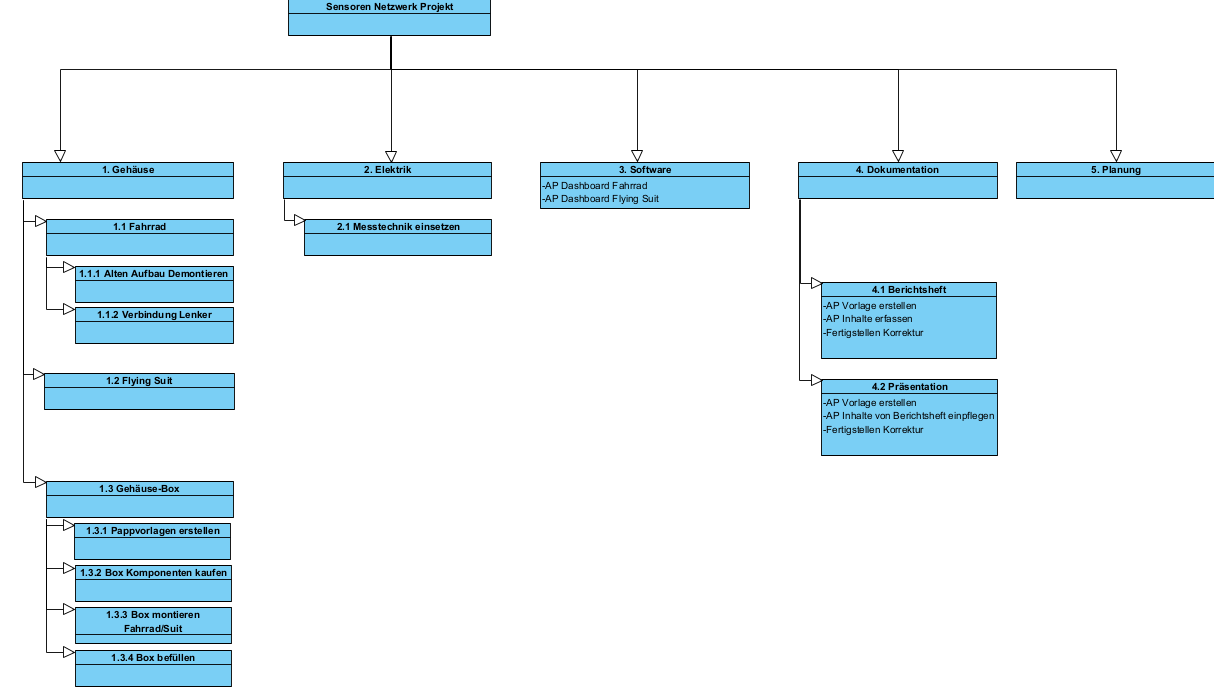
\includegraphics[width=1.0\textwidth, keepaspectratio]{plan.png}
        \caption[Aufgaben (Abbildungsverzeichnis)]{Aufgaben
        %\cite{VLInkManual}
        }
        \label{fig:plan}
    \end{center}
\end{figure}


Aufgrund der Gruppenstärke von fünf Studenten erschien es sinnvoll zunächst eine Aufgabenverteilung und Aufteilung in Teams durchzuführen.
Nachdem sich jeder mit der Aufgabenstellung und den notwendigen theoretischen Grundlagen vertraut gemacht hatte geschah die Aufteilung in die Teams Fahrrad (Bellgardt, Menzel) und Flying Suit (Grote, Nerb, Ulit).
Zu einem späteren Zeitpunkt hat sich vom Team Flying Suit das Team Software (Grote) abgespaltet, siehe Abbildung \ref{fig:aufgabenverteilung}.

Diese Aufteilungen waren sinnvoll, um dem großen Umfang des Projekts gerecht werden zu können. Hierbei hat das Team Fahrrad in den Laboren von Professor Kuttner gearbeitet während das Team Flying Suit einen Teil ihrer Arbeiten, insbesondere die der Messungen bei Herrn Landuris in dessen Räumlichkeiten durchgeführt haben.

Um erarbeitete Konzepte, Lösungen u.ä. zwischen und innerhalb der Teams nutzen zu können wurde während des Projekts auf TeamDrive zugegriffen um Dateien zugänglich zu machen.
Zur Präsentation des Projekts im Hörsaalrahmen wurde eine geteilte Powerpoint verwendet. Dieser Bericht wurde in Latex erstellt.

\begin{figure}[h]
    \begin{center}
        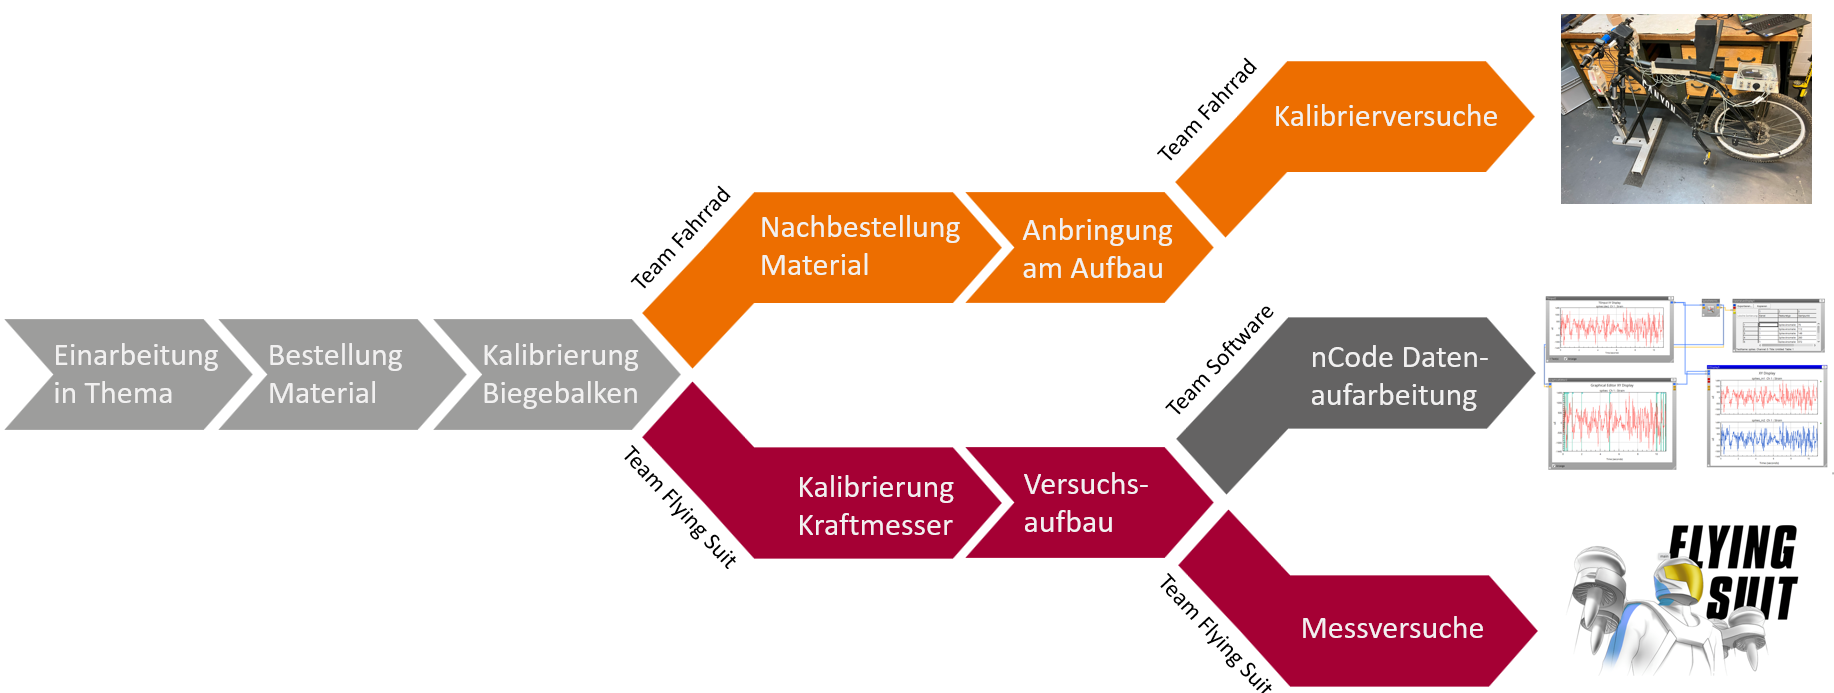
\includegraphics[width=1\textwidth, keepaspectratio]{aufgabenverteilung.png}
        \caption[Aufgabenverteilung Entwicklungsteams (Abbildungsverzeichnis)]{Aufgabenverteilung Entwicklungsteams
        %\cite{VLInkManual}
        }
        \label{fig:aufgabenverteilung}
    \end{center}
\end{figure}
\chapter{Theoretische Grundlagen}


\section{Drahtlose Sensornetzwerke und der V-Link 200 \(Menzel\)}

Dies soll durch die Verwendung des VLINK200 Nodes der Herstellers LORD/HBK stattfinden.
Dieses Unternehmen bietet Lösungen für drahtlose Sensornetzwerke an. Diese werden in der Industrie und dem Internet of Things, sowie auch in der Forschung und im Maschinen und Anlagenbau verwendet.
Dort wird sie vor allem im Bereich der predictive Maintenance eingesetzt.
Der Node verfügt über 8 Eingänge, 4 ±156mV Differenzeingänge und 4 ± 156mV Single-Ended Eingänge.
Er gewährleistet eine verlustfreie Datenübertragung sowie auch die Speicherung von Messdaten.
Man kann den Node über interne, austauschbare Batterien und externe Akkus betreiben.

\begin{figure}[h]
    \begin{center}
        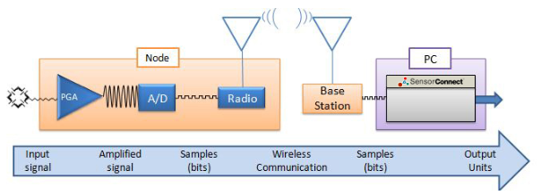
\includegraphics[width=1\textwidth, keepaspectratio]{lord_wireless.png}
        \caption[LORD drahtlose Übertragung (Abbildungsverzeichnis)]{LORD drahtlose Übertragung
        \cite{VLInkManual}
        }
        \label{fig:lordwireless}
    \end{center}
\end{figure}

Abbildung \ref{fig:lordwireless} zeigt die Funktionsweise der drahtlosen Datenübertragung.
Ein an das Node angeschlossener Sensor wird innerhalb des Nodes verstärkt und digitalisiert.
Anschließend werden die Messdaten vom Node drahtlos an eine Base Station gesendet welche mit einem Laptop verbunden ist.
Dort kann durch die Software SensorConnect auf den Node zugegriffen werden und dessen Daten visualisiert oder weiter verarbeitet werden.


Abbildung \ref{fig:lordproducts} zeigt einen Teil der Produktpalette.
Als Gateway wurde von uns der dort gezeigte USB Stick genutzt.
Insgesamt wurden uns zwei VLINK 200 Node, und ein USB Stick zur Verfügung gestellt was in der späten Projektphase teilweise zu Problemen führte,
siehe \ref{sec:probleme} \nameref{sec:probleme}.

\begin{figure}[h]
    \begin{center}
        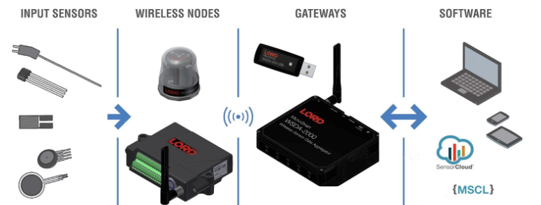
\includegraphics[width=1\textwidth, keepaspectratio]{lord_products.png}
        \caption[LORD Produkte (Abbildungsverzeichnis)]{LORD Produkte
        \cite{VLInkManual}
        }
        \label{fig:lordproducts}
    \end{center}
\end{figure}


\section{Dehnungsmessstreifen und Messprinzipien \(Bellgardt\)}
Dehnungsmessstreifen (DMS) sind sensorische Elemente, die zur Messung von mechanischen Dehnungen in Bauteilen eingesetzt werden. Das Wirkprinzip beruht auf der Änderung des elektrischen Widerstands eines metallischen oder halbleitenden Messgitters, wenn es durch eine mechanische Belastung gedehnt oder gestaucht wird. Diese Widerstandsänderung ist direkt proportional zur mechanischen Dehnung des Materials, auf das der DMS aufgeklebt ist. 
Das Messprinzip basiert auf dem Zusammenhang zwischen der mechanischen Dehnung und der Widerstandsänderung des DMS. Wird das Trägermaterial belastet, verändert sich seine Geometrie, wodurch sich auch die Länge und der Querschnitt des Messgitters ändern. Dies beschreibt die Gleichung des elektrischen Widerstands:

$R = \rho \cdot \frac{l}{A}$,

mit $\rho$ als spezifischem Widerstand, l als Länge und A als Querschnitt ergibt sich, dass eine Längenzunahme bei gleichzeitiger Verringerung des Querschnitts zu einer Erhöhung des Widerstands führt. Um diese Widerstandsänderung messbar zu machen, wird häufig eine Wheatstone-Brücke verwendet, die Spannungsänderungen proportional zur Dehnung des Materials erfasst.
DMS finden breite Anwendung in der experimentellen Spannungsanalyse, der Kraftmessung und der Strukturüberwachung in verschiedenen Ingenieurbereichen. Durch ihre hohe Empfindlichkeit und Präzision sind sie essenzielle Sensoren zur mechanischen Zustandsüberwachung von Bauteilen und Maschinen.










\newpage{}
\section{Viertel\-, Halb\- und Vollbr\"uckenschaltungen für DMS \(Bellgardt\)}
Zur präzisen Messung mechanischer Dehnungen werden Dehnungsmessstreifen häufig in Form einer Wheatstone-Brücke verschaltet. Dabei gibt es drei Hauptkonfigurationen: die Viertelbrücke, die Halbbrücke und die Vollbrücke, die sich in ihrer Empfindlichkeit, Temperaturkompensation und Messgenauigkeit unterscheiden.

\subsection{Viertelbrückenschaltung}
Die einfachste Form ist die Viertelbrückenschaltung (siehe Abbildung \ref{fig:fab1} links), bei der nur ein einzelner DMS als aktiver Widerstand in die Brückenschaltung integriert wird, während die anderen drei Widerstände passive Referenzwiderstände sind. Die Widerstandsänderung des DMS führt zu einer Veränderung der Brückenspannung, die als Messsignal ausgewertet wird. Da nur ein DMS aktiv zur Messung beiträgt, ist die Empfindlichkeit dieser Schaltung vergleichsweise gering. Zudem sind Temperaturkompensation und Störunterdrückung begrenzt, da äußere Einflüsse nicht ausreichend ausgeglichen werden. Die Viertelbrücke wird häufig in einfachen Spannungsmessungen eingesetzt, wenn nur geringe Genauigkeitsanforderungen bestehen.

\subsection{Halbbrückenschaltung}
Eine präzisere Alternative stellt die Halbbrückenschaltung  (siehe Abbildung \ref{fig:fab1} mittig) dar, bei der zwei DMS in die Brückenschaltung eingebaut sind. Diese werden oft so angeordnet, dass einer gedehnt und der andere gestaucht wird, wodurch sich ihre Widerstandsänderungen addieren und das Ausgangssignal verstärken. Dadurch erhöht sich die Messgenauigkeit im Vergleich zur Viertelbrücke. Gleichzeitig verbessert sich die Temperaturkompensation, da beide DMS denselben Umgebungseinflüssen ausgesetzt sind und sich temperaturbedingte Widerstandsänderungen teilweise gegenseitig aufheben. In diesem Projekt wurde hauptsächlich die Halbbrückenschaltung verwendet.

\subsection{Vollbrückenschaltung}
Die höchste Präzision und Empfindlichkeit bietet die Vollbrückenschaltung  (siehe Abbildung \ref{fig:fab1} rechts), bei der vier aktive DMS in die Wheatstone-Brücke integriert sind. Dabei befinden sich zwei DMS in einem gedehnten und zwei in einem gestauchten Zustand, wodurch sich ihre Widerstandsänderungen vollständig addieren und ein maximales Ausgangssignal erzeugt wird. Die Vollbrücke bietet nicht nur die beste Messgenauigkeit, sondern auch eine optimale Temperaturkompensation, da sich externe Temperatureinflüsse auf alle vier DMS gleichmäßig auswirken und somit weitgehend eliminiert werden.
Ein Vergleich dieser Brückenkonfigurationen findet sich zusammengefasst in Tabelle \ref{tbl:dms_schaltungen}


\bgroup
\def\arraystretch{2}
\begin{table}[h]
\centering
\begin{tabular}{|p{0.25\linewidth}|p{0.25\linewidth}|p{0.25\linewidth}|p{0.25\linewidth}|}
\hline
Schaltung & Anzahl aktiver DMS & Empfindlichkeit & Anwendung \\ \hline
Viertelbrücke & 1 & Gering & Einfache Dehnungsmessung \\ \hline
Halbbrücke & 2 & Mittel & Biegung, Torsion, Kraftmessung \\ \hline
Vollbrücke & 4 & Hoch & Hochpräzise Messung, industrielle Sensorik \\ \hline
\end{tabular}
\caption{Vergleich verschiedener DMS-Schaltungen}
\label{tbl:dms_schaltungen}
\end{table}
\egroup


\begin{figure}[h]
    \begin{center}
        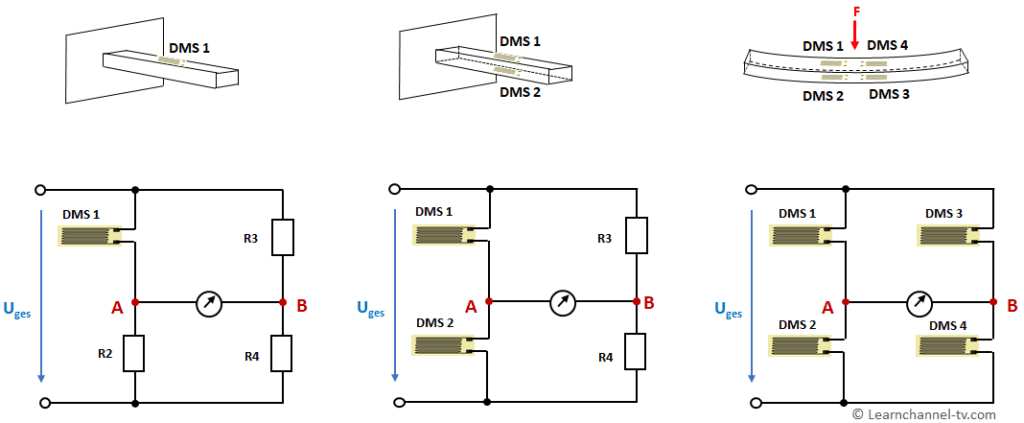
\includegraphics[width=1.0\textwidth, keepaspectratio]{fab1.png}
        \caption[DMS in Viertel\- Halb\- und Vollbr\"uckenkonfiguration (Abbildungsverzeichnis)]{DMS in Viertel\- Halb\- und Vollbr\"uckenkonfiguration
        \footcite{https://learnchannel-tv.com/wp-content/uploads/2020/12/Wheatstone-DMS-Messbrucke-Viertel-Halb-Vollbrucke-1024x423.png}
        }
        \label{fig:fab1}
    \end{center}
\end{figure}






\section{Mechanische Belastungen \(Bellgardt\)}
Mechanische Belastungen entstehen, wenn äußere Kräfte oder Momente auf ein Bauteil einwirken und Spannungen sowie Verformungen im Material verursachen. Je nach Art der Beanspruchung unterscheidet man verschiedene Belastungsformen, die jeweils charakteristische Spannungs- und Dehnungszustände hervorrufen. Besonders relevant für die Dehnungsmessung sind Biegung, Torsion und axiale Kraftbeanspruchung, da sie mit Hilfe von Dehnungsmessstreifen (DMS) präzise erfasst werden können.

\begin{figure}[h]
    \begin{center}
        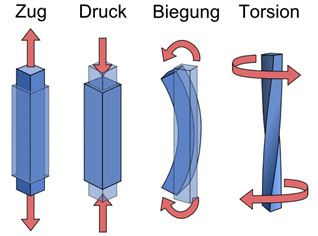
\includegraphics[width=0.5\textwidth, keepaspectratio]{fab2.png}
        \caption[Verschiedene Krafteinwirkungen (Abbildungsverzeichnis)]{Verschiedene Krafteinwirkungen
        \footcite{https://www.maschinenbau-wissen.de/bilder/skripte/mechanik/belastungsarten-03.PNG}
        }
        \label{fig:fab2}
    \end{center}
\end{figure}
\subsection{Biegung: Verformung durch einwirkende Kräfte}
Bei einer Biegebelastung wird ein Bauteil durch äußere Kräfte oder Momente gekrümmt. Dies führt zu einer Biegespannung, die entlang des Querschnitts eine typische Spannungsverteilung erzeugt: Auf der einen Seite des Bauteils tritt eine Dehnung (Zugspannung) auf, während die gegenüberliegende Seite gestaucht wird (Druckspannung). Dazwischen liegt die neutrale Faser, eine Linie oder Fläche ohne Längenänderung.
Zur Messung von Biegespannungen werden DMS typischerweise auf der Ober- und Unterseite des Bauteils angebracht. Eine Halbbrücken- oder Vollbrückenschaltung ist besonders vorteilhaft, da sie die Widerstandsänderungen der DMS kombiniert und sowohl die Empfindlichkeit als auch die Temperaturkompensation verbessert. Einsatzgebiete sind etwa: Bauwerksüberwachung, Maschinenbau und die Belastungsprüfung von Bauteilen.

\subsection{Torsion: Drehmomente und Schubspannungen}
Torsion tritt auf, wenn ein Bauteil um seine Längsachse verdreht wird, beispielsweise bei Antriebswellen oder Schraubverbindungen. Dabei entstehen Schubspannungen, die unter einem ±45°-Winkel zur Achse verlaufen.
Zur Messung von Torsionsbeanspruchungen werden DMS in einer schrägen Anordnung (meist in ±45°-Orientierung) angebracht, sodass sie die maximalen Schubspannungen erfassen. Eine Halbbrücke mit zwei DMS oder eine Vollbrücke mit vier DMS ermöglicht eine genaue Bestimmung des aufgebrachten Drehmoments. Eine Messung der Torsion wird oft für die Überwachung von rotierenden Maschinen, Fahrzeugantrieben und industriellen Wellen genutzt.

\subsection{Zug- und Druck}
\todo{}





\section{Biegebalken \(Menzel\)}
Die Entwicklung einer neuen Messtechnik für das Fahrrad und den Flying Suit stellt eine komplexe Aufgabe da.
Dies beinhaltet die Planung und Bestellung nötiger Materialien und die Anbringung dieser am jeweiligen Aufbau.
Um sicherzustellen, dass die zu entwickelnde technische Umsetzung möglich ist, wurde das Zusammenspiel von Node und Dehnungsmessstreifen zunächst am einfacheren Aufbau eines Biegebalkens getestet.


\subsection{Aufbau des Biegebalkens}
Auf der Ober- und Unterseite des Biegebalkens sind Dehnungsmessstreifen angebracht um die beim aufbringen eines Gewichts entstehende Dehnung messen zu können.
Dies wurde mit verschiedenen Gewichten und in verschiedenen Einheiten durchgeführt.
\begin{figure}[h]
    \begin{center}
        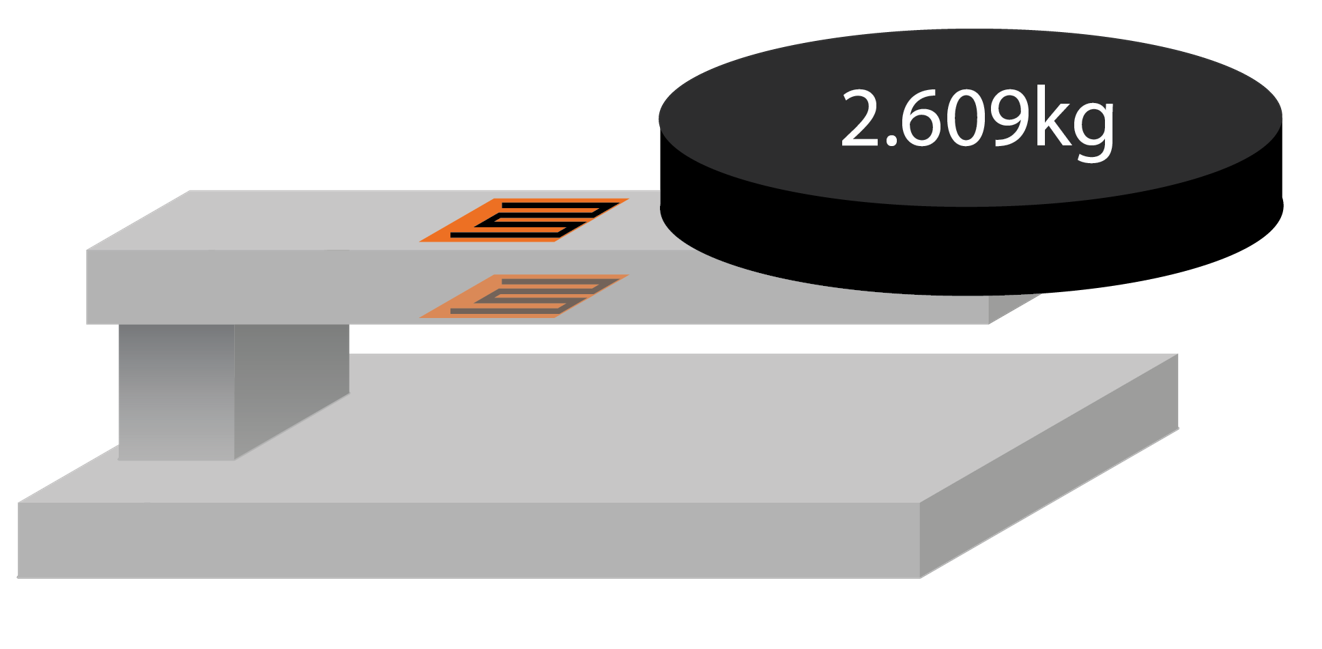
\includegraphics[width=0.5\textwidth, keepaspectratio]{biegebalken_grafik.png}
        \caption[Biegebalken Schema (Abbildungsverzeichnis)]{Biegebalken Schema
        %\cite{VLInkManual}
        }
        \label{fig:biegebalkenschema}
    \end{center}
\end{figure}

\subsection{Wahl des Messverfahrens}
Um Messungen durchführen zu können bieten sich verschiedene Verfahren an.
Die in der Software SensorConnect verfügbaren und für uns relevanten Verfahren sind die Shunt-, Field-, und Sensitivity(geometriebasierte)-kalibrierung.
Die Beschreibung sowie die Vor- und Nachteile dieser Verfahren sind in \ref{tbl:verfahren} \nameref{tbl:verfahren} dargestellt.
Um die theoretische Grundlage für den Aufbau des Fahrrads und des Flying Suits zu schaffen wurde sich beim Biegebalken für die Wahl des mV/V Messverfahrens entschieden.

\bgroup
\def\arraystretch{2}
\begin{table}[h]
\centering
\begin{tabular}{|p{0.25\linewidth}|p{0.25\linewidth}|p{0.25\linewidth}|p{0.25\linewidth}|}
\hline
Verfahren & Beschreibung & Vorteil & Nachteil\\ \hline
Shunt Kalibrierung & Interner (Shunt) Widerstand wird zur DMS-Brücke geschaltet. Es wird eine definierte Dehnung simuliert, um die Messkette zu überprüfen.
& schnell, einfach & Simuliert keine echte mech. Belastung, nur elektrische Effekte
\\ \hline
Field Kalibrierung & Messung von realer mech. Belastung mit Referenzlast

& Wenn Last bekannt ist, kann man sehr genau messen.
& Definierte Belastung der Struktur notwendig

\\ \hline
Geometriebasierte Kalibrierung (mV/V)
 & Berechnung für Software basierend auf Materialparametern und Geometrie


& Ermöglicht eine Abschätzung und Vergleich zwischen erwarteten und gemessenen Werten

& Abweichungen bei ungenauen Materialparametern möglich


\\ \hline

\end{tabular}
\caption{Messverfahren}
\label{tbl:verfahren}

\end{table}
\egroup


\subsection{Berechnung der Sensitivity}
Um eine Messung am Biegebalken durchführen zu können wurde zunächst die Sensitivity mathematisch berechnet.
Sie basierst auf der Geometrie des Biegebalkens, sowie des zu erwartendem maximalen Gewicht und wird als Parameter in SensorConnect eingegeben.
Sie stellt den gemessenen Wert in mV/V bei Maximalbelastung dar.
Aufgrund der einfachen Geometrie des Biegebalkens ist dies ein wichtiger Schritt, bevor diese für die komplexere Geometrie des Fahrradlenkers oder des Gestells des Flying Suits berechnet wird.

In der folgenden Berechnung wird für den Parameter n der Wert 2 verwendet, da es sich um die Anzahl der angebrachten DMS und die daraus resultierende Brückenkonfiguration handelt.
Der Parameter k ist durch die verwendeten DMS gegeben. Als maximale Last dient eine Hantelscheibe mit einem Gewicht von 2.609kg.



Maße des Biegebalkens:
\[
l = 117 \text{ mm}, \quad b = 19.8 \text{ mm}, \quad h = 2.94 \text{ mm}
\]
Maximale Last:
\[
M = 2.609 \text{ kg}
\]

\subsection*{Berechnung des Widerstandsmoments}
\[
W_x = \frac{b h^2}{6}
\]
Einsetzen der Werte:
\[
W_x = \frac{19.8 \times 2.94^2}{6} = 28.52 \text{ mm}^3
\]

\subsection*{Berechnung des Biegemoments}
\[
M_b = F \times l
\]
\[
M_b = 2.609 \times 9.81 \times 117mm = 2994.53 \text{ Nmm}
\]

\subsection*{Berechnung der Spannung}
\[
\sigma = \frac{M_b}{W_x}
\]
\[
\sigma = \frac{2994.53}{28.52} = 104.99 \text{ N/mm}^2
\]

\subsection*{Berechnung der Dehnung}
\[
\varepsilon = \frac{\sigma}{E}
\]
Mit \(E = 210000 \text{ N/mm}^2\):
\[
\varepsilon = \frac{104.99}{210000} = 0.499\times 10^{-3}
\]

\subsection*{Berechnung der Brückenausgabe}
\[
\frac{U_M}{U_B} = \frac{n}{4} \times k \times \varepsilon
\]
Mit \( n = 2 \), \( k = 2.01 \):
\[
\frac{U_M}{U_B} = \frac{2}{4} \times 2.01 \times 0.499 \times 10^{-3}
\]
\[
\frac{U_M}{U_B} = 0.000502 \text{ V/V} = 0.5 \text{ mV/V}
\]

Mit der berechneten Sensitivity wurden mehrere Messungen durchgeführt.
Die erste Messung wurde mit einem Gewicht von 2.609kg durchgeführt und in MPa gemessen, siehe \ref{tbl:biegebalkenmessungeins} \nameref{tbl:biegebalkenmessungeins}.

\bgroup
\def\arraystretch{2}
\begin{table}[h]
\centering
\begin{tabular}{|p{0.33\linewidth}|p{0.33\linewidth}|p{0.33\linewidth}|}
\hline
Gegeben & Gemessen & Abweichung \\ \hline
105MPa (2.609kg) & 120MPa (2.8kg) & +14\% \\ \hline
\end{tabular}
\caption{Messung 1 mit Maximalgewicht, [MPa]}
\label{tbl:biegebalkenmessungeins}

\end{table}
\egroup

Die zweite Messung wurde mit verschiedenen Gewichten getestet und in N gemessen, siehe \ref{tbl:biegebalkenmessungzwei} \nameref{tbl:biegebalkenmessungzwei}.
\bgroup
\def\arraystretch{2}
\begin{table}[h]
\centering
\begin{tabular}{|p{0.33\linewidth}|p{0.33\linewidth}|p{0.33\linewidth}|}
\hline
Gegeben & Gemessen & Abweichung \\ \hline
0N (0kg) & 0.2N (0.02kg) & - \\ \hline
3.9N (0.4kg) & 4.6N (0.46kg) & +17.9\%  \\ \hline
24.5N (2.609kg) & 27.6N (2.81kg)  & +12.6\% \\ \hline
\end{tabular}
\caption{Messung 2, [N]}
\label{tbl:biegebalkenmessungzwei}

\end{table}
\egroup





\chapter{Systemaufbau und Umsetzung}

\section{Technikstand Fahrrad \(Bellgardt, Menzel\)}
\label{sec:technikstandfahrrad}
Der Fahrradaufbau dient zur Erfassung von Kräften am Fahrradlenker, indem mechanische Größen in elektrische Signale umgewandelt werden. Dazu werden Dehnungsmessstreifen (DMS) verwendet, die auf relevante Bauteile aufgeklebt werden, um dort auftretende Verformungen zu erfassen. In einer Messbox befindet sich die Messtechnik. Diese zeichnet über die Zeit dann die Belastung auf. Insgesamt befinden sich an dem Lenker 8 DMS. Auf jeder Lenkerseite gibt es jeweils zwei DMS welche als Halbbrücke geschaltet, die Kräfte in horizontaler oder vertikaler Richtung messen. 
Abbildungen \ref{fig:fab3} und \ref{fig:fab4} zeigen den alter Aufbau des Fahrrads.
Um den alten Versuchsaufbau bei Bedarf wieder herstellen zu können musste dieser genau dokumentiert werden.
Dies geschah durch das Beschriften der in der Lenkerbox befindlichen Kabel, siehe \todo{Anhang}


An dem bisherigen Aufbau wurden folgende Optimierungsmöglichkeiten erkannt:
\begin{itemize}
    \item Bisheriger Aufbau am Fahrrad kabelgebunden (USB-Kabel zu PC)
    \item Keine Zugentlastung an der Lenkerbox
    \item Nicht spritzwassergeschützt
    \item Zwischenplatine benötigt
    \item Kontaktierung durch Verschraubung
\end{itemize}

\begin{figure}[h]
    \begin{center}
        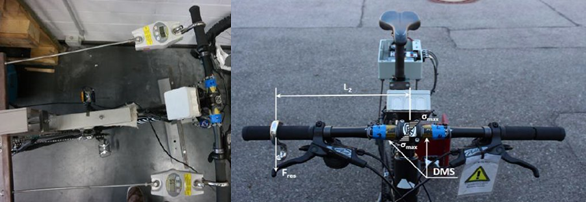
\includegraphics[width=1.0\textwidth, keepaspectratio]{fab3.png}
        \caption[Alter Aufbau des Fahrrads, Lenker (Abbildungsverzeichnis)]{Alter Aufbau des Fahrrads, Lenker
        \footcite{Rechter Teil des Bildes: Praktikum Schwingbruchgefaehrdete Bauteile sicher dimensionieren und betreiben
        }
        }
        \label{fig:fab3}
    \end{center}
\end{figure}


\begin{figure}[h]
    \begin{center}
        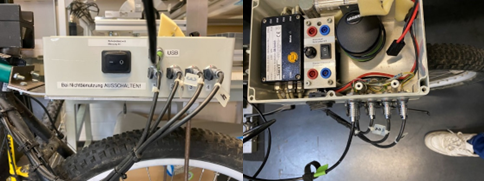
\includegraphics[width=1.0\textwidth, keepaspectratio]{fab4.png}
        \caption[Alter Aufbau des Fahrrads, Messbox (Abbildungsverzeichnis)]{Alter Aufbau des Fahrrads, Messbox}
        %\footcite{Rechter Teil des Bildes: Praktikum Schwingbruchgefaehrdete Bauteile sicher dimensionieren und betreiben
        %}
        
        \label{fig:fab4}
    \end{center}
\end{figure}



\section{Wahl der Komponenten \(Nerb, Ulit\)}


\section{Einbau des V\-Link 200 in ein spritzwassergesch\"utztes Geh\"ause \(Nerb, Ulit\)}
\section{Entwurf der Schaltung und Platine}




\subsection{Umschalter f\"ur Halb\- und Vollbr\"uecke \(Nerb, Ulit\)}
\subsection{Vollbr\"uckenschaltung f\"ur zwei DMS \(Nerb, Ulit\)}

\newpage{}
\subsection{Platinendesign Fahrrad \(Bellgardt, Menzel\)}
Zu Beginn sind wir davon ausgegangen, dass die DMS direkt mit der neuen Messtechnik verbunden werden können, siehe Abbildung \ref{fig:fab5}.
\begin{figure}[h]
    \begin{center}
        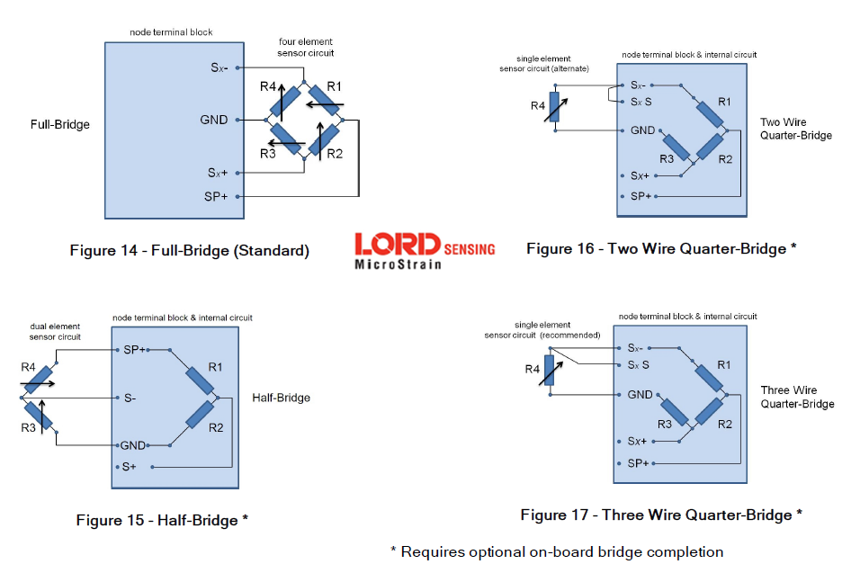
\includegraphics[width=0.9\textwidth, keepaspectratio]{fab5.png}
        \caption[LORD Konfigurationen der Brücken (Abbildungsverzeichnis)]{LORD Konfigurationen der Brücken}
        \footcite{VLInkManual
        }
        
        \label{fig:fab5}
    \end{center}
\end{figure}

Da dies nicht möglich ist, haben wir als Lösung eine Zwischenplatine konstruiert, welche die DMS mit zwei Widerständen zur Halbbrücke ergänzt, siehe Abbildung \ref{fig:fab6}.

\begin{figure}[h]
    \begin{center}
        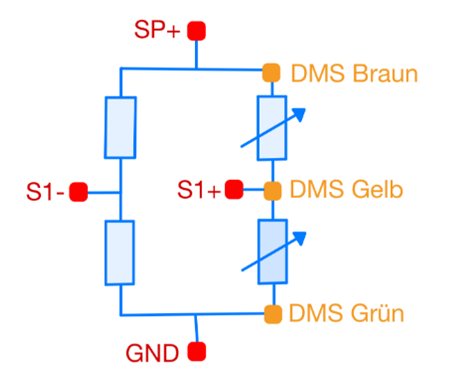
\includegraphics[width=0.4\textwidth, keepaspectratio]{fab6.png}
        \caption[Schaltplan Protoyp Platine (Abbildungsverzeichnis)]{Schaltplan Protoyp Platine}
        %\footcite{VLInkManual
        %}
        
        \label{fig:fab6}
    \end{center}
\end{figure}

Für die Messtechnik sieht dies nun aus wie eine Vollbrücke. Um uns das Wirkungsprinzip und die Funktionsfähigkeit zu verdeutlichen, wurde die Schaltung für den Biegebalken konstruiert.
Der Mittelabgriff des Biegebalkens ist dabei die gelbe Ader. Die Versorgungsapannung von 4,096 V wird durch die Messtechnik vorgegeben und liegt zwischen den Kontakten SP+ und GND an. Der Brückenausgang wird zwischen S1- und S1+ gemessen. Hierüber wird die Belastung der Brücke durch Dehnung der DMS in eine Spannung zwischen S1- und S1+ dargestellt
\subsubsection{Der erste Prototyp}
Basierend auf dem ersten Schaltungsplan wurde dann eine Prototyp-Platine erstellt. Die Platine basiert auf einer Lochplatine. Die verwendeten Widerstände sind 120 Ohm-Metallschichtwiderstände mit einer Abweichung von 1 \%. Der Prototyp wurde am Biegebalken getestet.
\begin{figure}[h]
    \begin{center}
        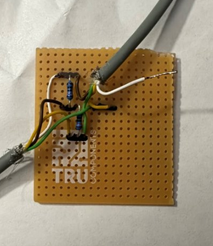
\includegraphics[width=0.4\textwidth, keepaspectratio]{fab7.png}
        \caption[Prototyp Platine mit der Ergänzung der DMS zur Halbbrücke (Abbildungsverzeichnis)]{Prototyp Platine mit der Ergänzung der DMS zur Halbbrücke}
        %\footcite{VLInkManual
        %}
        
        \label{fig:fab7}
    \end{center}
\end{figure}

\subsubsection{Platinenplanung der Lenkerbox}
\todo{fabian reihenfolge erklaerung kicad sinnvoll}
Der Alte Aufbau hat einige Eigenschaften, die durch den neuen Aufbau verbessert wurden. So wurde der alte Aufbau auf einer Lochplatine realisiert.
Zudem wurde die Verbindung der Platine mit Schraubklemmen gelöst. Der Aufbau ist nicht spritzwassergeschützt und die verwendeten Leitungen sind nicht geschirmt.
Die alte Lenkerbox besitzt zudem keine Zugentlastung der Leitungen der DMS Streifen. Es gibt auch keine Zugentlastung der Leitungen zur Messtechnik. 
\begin{figure}[h]
    \begin{center}
        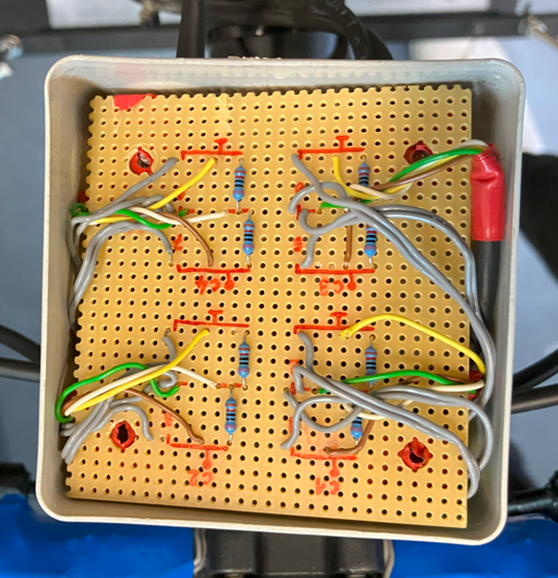
\includegraphics[width=0.3\textwidth, keepaspectratio]{fab8.png}
        \caption[Alte Platine in der alten Lenkerbox (Abbildungsverzeichnis)]{Alte Platine in der alten Lenkerbox}
        %\footcite{VLInkManual
        %}
        
       \label{fig:fab8}
    \end{center}
\end{figure}

Viele der angemerkten Punkte konnten verbessert werden. Hierzu wurde zunächst der Schaltplan in der Software KiCad\cite{KiCadWebsite} eingepflegt.
\todo{fabian reihenfolge erklaerung kicad sinnvoll}

KiCAD ist ein freies Tool, mit welchem man Platinen planen kann. Nach dem erfolgreichen Test der Prototyp Platine an dem Biegbalken wurde die Schaltung hochskaliert. Der Hauptunterschied im Anschluss der DMS des Biegebalkens und denen des Fahrrads besteht darin, dass der Mittelabgriff am Fahrrad durch die weißen DMS bereitgestellt wird.
\begin{figure}[h]
    \begin{center}
        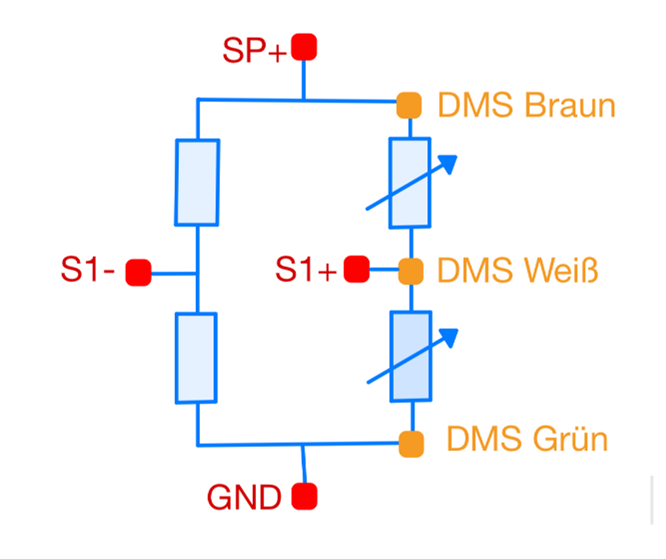
\includegraphics[width=0.4\textwidth, keepaspectratio]{fab9.png}
        \caption[Schaltungsplan Fahrrad (Abbildungsverzeichnis)]{Schaltungsplan Fahrrad}
        %\footcite{VLInkManual
        %}
        
        \label{fig:fab9}
    \end{center}
\end{figure}

\subsubsection{Planung der Schaltung mit KiCAD}
In der Software KiCAD\cite{KiCadWebsite} wurde zunächst ein Schaltplan erstellt, siehe \ref{fig:fab11}.
\begin{figure}[h]
    \begin{center}
        
\includegraphics[width=0.2\textwidth, keepaspectratio]{fab10.png}
        \caption[KiCad Software Logo (Abbildungsverzeichnis)]{KiCad Software Logo}
        \cite{KiCadWebsite}
        \label{fig:fab10}
    \end{center}
\end{figure}


Dieser stellt 4 Halbbrücken dar.
Auf der Platine werden pro Halbbrücke je zwei Widerstände angebracht. Die befinden sich in Form ihrer Kontakte auf der Platine.
Basierend auf dem Schaltplan (siehe Anhang \ref{sec:schaltplan2}) wurde dann die Platine zunächst entsprechend Ihrer Abmessungen für das Gehäuse simuliert (siehe \ref{fig:fab12}) und anschließend gedruckt. Die fertige Platine ist in der Abbildung \ref{fig:fab13}zu sehen. Sie besitzt die Maße des Gehäuses. Zudem verfügt die Platine über 4 zusätzliche Bohrungen, um sie besser im Gehäuse befestigen zu können. 
\begin{figure}[h]
    \begin{center}
        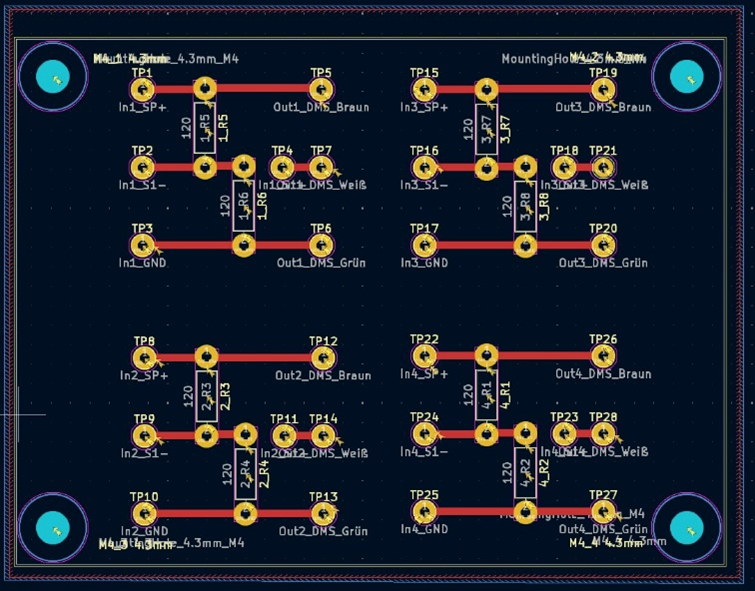
\includegraphics[width=0.4\textwidth, keepaspectratio]{fab11.png}
        \caption[Planung Lenkerplatine (Abbildungsverzeichnis)]{Planung Lenkerplatine}
        %\footcite{www.kicad.org}
        \label{fig:fab11}
    \end{center}
\end{figure}

\begin{figure}[h]
    \begin{center}
        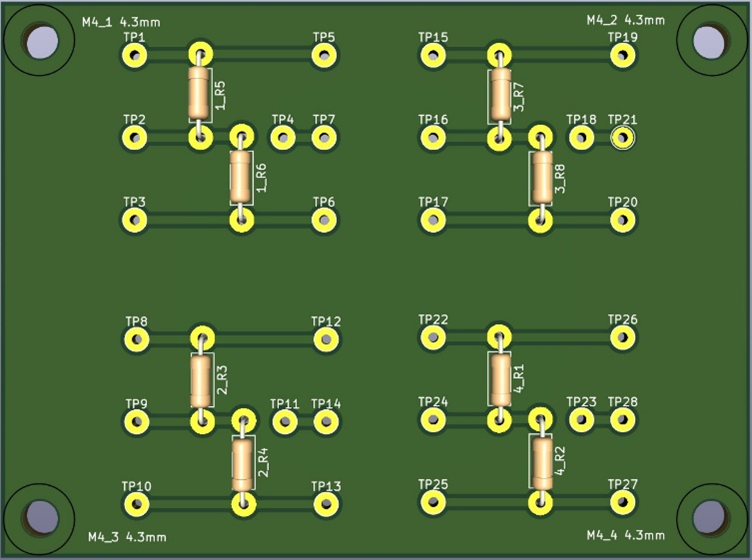
\includegraphics[width=0.4\textwidth, keepaspectratio]{fab12.png}
        \caption[Simulation der Lenkerplatine (Abbildungsverzeichnis)]{Simulation der Lenkerplatine}
        %\footcite{www.kicad.org}
        \label{fig:fab12}
    \end{center}
\end{figure}

\begin{figure}[h]
    \begin{center}
        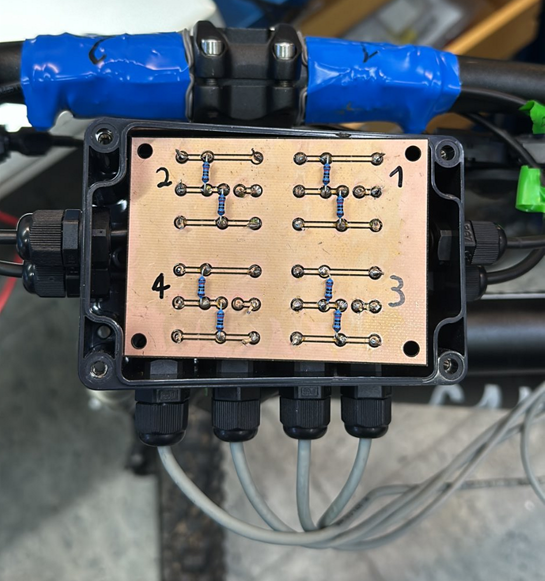
\includegraphics[width=0.4\textwidth, keepaspectratio]{fab13.png}
        \caption[Fertig installierte Lenkerplatine (Abbildungsverzeichnis)]{Fertig installierte Lenkerplatine}
        %\footcite{www.kicad.org}
        \label{fig:fab13}
    \end{center}
\end{figure}





\newpage{}

\subsection{Platinendesign Suit \(Nerb, Ulit\)}
\section{Herstellung der Acrylplatte f\"ur die Geh\"auseintegration \(Nerb, Ulit\)}
\section{Montage und Verbindung der DMS \(Nerb, Ulit\)}

\chapter{Durchgeführte Versuche und Lösungswege}
\label{cha:durchführung}
\todo{}
\chapter{Ergebnisse}
\label{cha:ergebnisse}
\todo{}
\chapter{Software und Datenverarbeitung}

\section{Auslesen der Messwerte}
\section{Schnittstellen und Datenprotokoll}
\section{Darstellung und Visualisierung der Messwerte}

\chapter{Fazit}
\label{cha:fazit}
\todo{}
%\chapter{Fazit}
\label{cha:fazit}
\todo{}






%\input{chapters/glossary}


% ------------------
% |    Appendix    |
% ------------------
\appendix

\appendix
\chapter{Anhang}
\label{cha:anhang}


\section{Anhang 1}


% ----------------------
% |    Bibliography    |
% ----------------------
\printbibheading[title={Literaturverzeichnis}] % Main heading for the bibliography

\printbibliography[heading=subbibliography, type=book, title={Bücher}]
\printbibliography[heading=subbibliography, type=online, title={Online Quellen}]
\printbibliography[heading=subbibliography, type=source, title={Verweise}]


\end{document}
